\chapter{Introduction and Getting Started}

\section{Introduction and Features}

CoolSPICE, from CoolCAD Electronics, LLC, is a full-featured simulation suite.  Its SPICE engine allows for mixed-level/mixed-signal circuit simulation. CoolSPICE is a complete suite including a graphical Schematics Editor, a text-based Netlist Editor and a Plotter for the results. Example circuits to demonstrate the devices and simulation features are also included in the package.

Features of CoolSPICE include:

\begin{itemize} 
	\item Standard SPICE models and analysis tools
	\item Silicon Carbide/Gallium Nitride MOSFETs
	\item Cryogenic CMOS simulation
	\item Simulation of radiation effects on CMOS operation
	\item High-power, high-temperature SiC device model libraries and simulation 
	\item Ability to set individual temperatures for devices in a design during simulation
	\item Self-consistent electrical/thermal simulations
	\item Niche device model libraries (e.g. rectennas, avalanche photodiodes...) and simulation	
	\item TCAD simulations for a variety of structures
\end{itemize}

The Student Version only includes the standard SPICE models and analysis tools.


\section{Installation and Setup}


\subsection{System Requirements}


\begin{itemize}
\item Windows XP or later,
\item Windows SDK 7.1 (included with the installer),
\item .NET Framework 4.5 or later (included with the installer),
\item Visual C++ 2010 SP1 x64, or later (included with the installer),
\item Visual C++ 2010 SP1 x86 (included with the installer),
\item WinSCP (optional, to directly run netlist files).
\end{itemize}

\subsection{Installation}

The free student version of CoolSPICE is available to download from CoolCAD's website. Simply go to 

\begin{center}
\fbox{\begin{minipage}{25em}
\begin{center}
http://coolcadelectronics.com/coolspice/
\end{center}
\end{minipage}}
\end{center}and enter your name and e-mail address.  You can opt in or out of joining the mailing list.  Click the {\colorbox{darkgreen}{\textcolor{white}{Download CoolSPICE}}} button for the download.  This sends you to the download page, where you can choose the version you wish.  When run, the installer creates shortcuts to the CoolSPICE Package on the desktop and in the Start menu.


\begin{wrapfigure}{r}{0.2\textwidth}
  \begin{center}
    
\includegraphics[width=0.15\textwidth]
	{./figures/getting_started_figures/CoolSPICEstudent_logo_shortcut.eps}
  \end{center}
  \caption{The desktop shortcut.}
  \label{fig_desktop_shortcut}
\end{wrapfigure}

\mymarginnote{Reinstalling Caution!} If you are reinstalling CoolSPICE or installing a new version, be aware that in the CoolSPICE default directories, all the files created by a previous use of the CoolSPICE installer will be overwritten.  For instance, if you have modified the circuits found in the \textsf{Ckts/}  directory, they will be overwritten by the default versions in the installer. It is a good idea to back up your circuits and netlists in another location before starting a new CoolSPICE installation.

To obtain the full commercial version, please contact CoolCAD Electronics at 
\begin{center}
\fbox{\begin{minipage}{25em}
\begin{center}
contact@coolcadelectronics.com\\
or +1-301-405-3363.
\end{center}
\end{minipage}}
\end{center}

\mymarginnote{Folder\\ locations} By default, CoolSPICE is installed in the folder \textsf{CoolSpice/} within the \textsf{My Documents/} folder of the Windows user account used for the installation.  \index{CoolSPICE!install locations} Within this folder, four subfolders will be created:

\begin{itemize}
\item \textsf{Ckts/}  This folder includes a collection of example circuits in schematic file format. These circuits can be saved under other names and edited to explore the capabilities of CoolSPICE.
\item \textsf{CoolCADSPICE/} This folder contains the executable files for the SPICE engine, the Schematics Editor, the Text Editor and the Plotter.
\item \textsf{Libraries/} This folder contains the schematic libraries used by the Schematics Editor.
\item \textsf{Models/} This folder contains SPICE models published by MOSIS (\textsf{MOSIS.txt}) and SPICE models for some other standard components (\textsf{StandardParts.txt}).
\end{itemize}

Within the \textsf{CoolCADSPICE/} folder, the subfolder \textsf{WinSCP/} is created. The open-source software \textbf{WinSCP} can optionally be installed here if the user wants the capability to run netlist files directly from the main console.  {\bf WinSCP} can be downloaded from
\vspace{-\parskip}
\begin{center}
\vspace{-\parskip}
\fbox{\begin{minipage}{\textwidth}
\begin{center}
{ http://coolcadelectronics.com/wp-content/uploads/2013/04/WinSCP.zip }
\end{center}
\end{minipage}}
\end{center}
and the extracted files from the zip archive should be placed in \\ \textsf{Documents/CoolSpice/CoolCADSPICE/WinSCP}\index{WinSCP!install location}.  

\section{Quick Start}

\label{sec_iags_quickstart} \index{CoolSPICE!quick start}

The CoolSPICE package is launched by double-clicking on the desktop shortcut or from the Start menu as \textsf{CoolSpice Package}  under the menu item \textsf{CoolSpice Package} under "All Programs."  The main console, as displayed in Figure \ref{fig_mainconsole}, comes up.  

\begin{SCfigure}[3.0][hbt]
  %\centering
    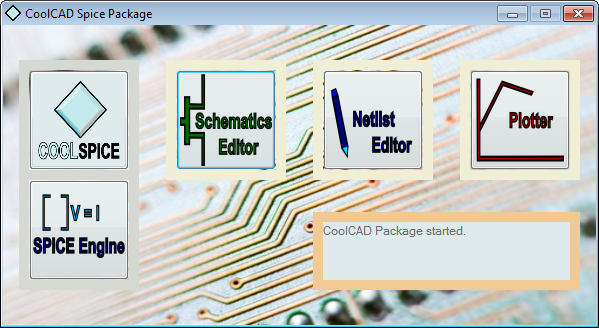
\includegraphics[width=0.55\textwidth]{./figures/getting_started_figures/CoolSPICE_mainconsole.png}
	\caption{{The main console of the CoolSPICE package.}}
  \label{fig_mainconsole}
\end{SCfigure}


\subsection{Building a Circuit}

On the main console, click on \textbf{Schematic Editor} to launch the Schematic Editor. By default, the Schematic Editor should open with frames which show the libraries and the selected symbol (when one is selected) to the left.  If these frames are not visible, click the \menuorbutton{Symbol Picker} button, which has the symbol \fbox{$\Omega$} (or press \makekey{F6}).  

For a fast-start example, we are going to build an inverter using the ON Semiconductor 0.5 $\mu$m technology and run a simulation to find its voltage and current transfer functions.  The MOSFET models are included in the built-in libraries of CoolSPICE.  Click on the ``+" symbol next to the MOSIS library to open up the list of components in this library.

\begin{SCfigure}[5.0][hbt]
    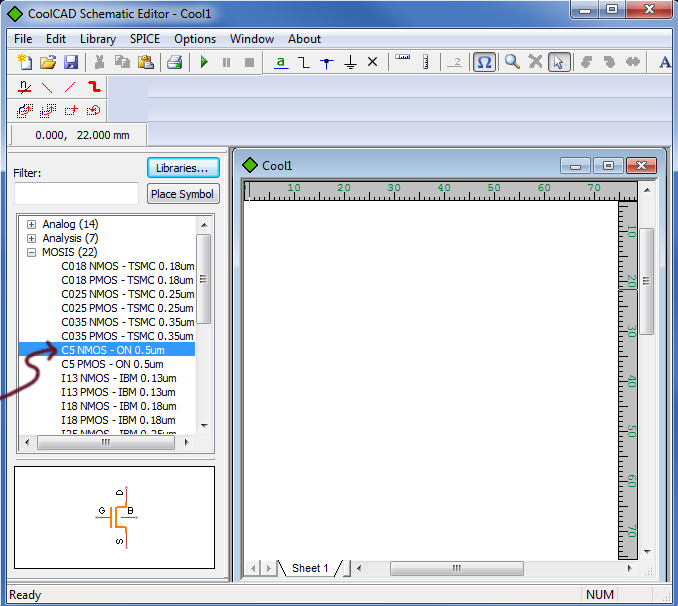
\includegraphics[width=0.55\textwidth]{./figures/getting_started_figures/CoolSPICE_emptySchematicEditor.png}
    \caption{{Schematic Editor with a model selected and ready.}}
  \label{fig_emptyschematiceditor}
\end{SCfigure}

\inserttip{Use the \textsf{\textsc{Esc}} key to cancel out of an action.} 

\mymarginnote{Inserting components} 
Double-clicking on the name of the required component (or single-clicking on the symbol which appears in the symbol frame) gives the user an instance of the component to place.  \index{Schematic Editor!component placement} It also opens up the \window{Options} for the component. \index{Schematic Editor!component options}  The user can place multiple instances of the same component until the place mode is cancelled by hitting the \textsf{\textbf{\textsc{Escape}}} key.  The \window{Options} disappears after the place mode is cancelled (or if the user clicks on an empty spot in the design area) and can be recalled by clicking on a component after placement.

\begin{SCfigure}[5.0][hbt]
    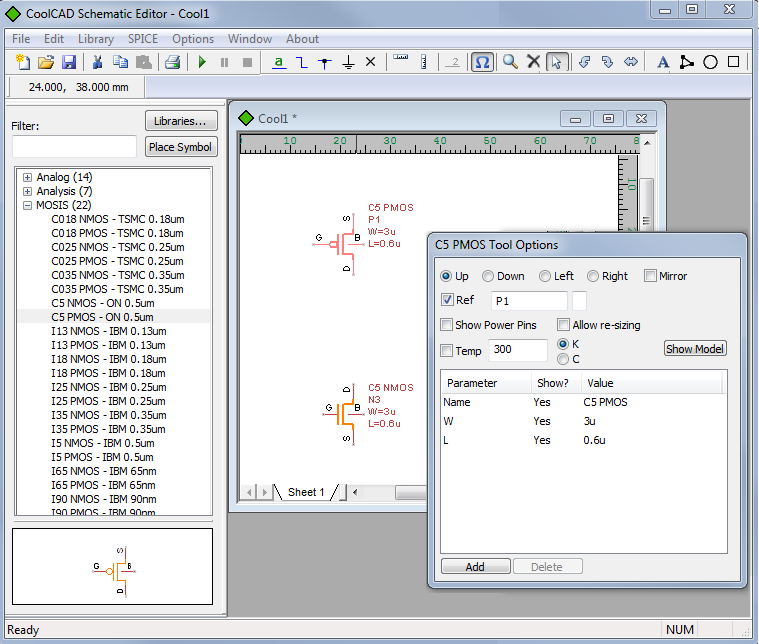
\includegraphics[width=0.55\textwidth]{./figures/getting_started_figures/CoolSPICE_SchematicEditorwithDevicesandOptions.png}
	\caption{{Schematic Editor with two components placed and the \textsf{Options} window.}}
  \label{fig_schematiceditor_devicesandoptions}
\end{SCfigure}

%\FloatBarrier
%\clearpage
%
\inserttip{Make sure all instances have distinct reference names. Avoid reference names with only numbers (e.g. ``42").} \mymarginnote{Component parameters} The component parameters can be changed by clicking on the value of the parameter in the \window{Options}.  As shown in Fig. \ref{fig_schematiceditor_changePMOSwidth}, here the width for the PMOS has been changed to 4.5 $\mu$m (by typing {\bf{\textsf{4.5u}}}).  The placement orientation and the instance reference name (\textbf{``Ref"}) for a component can also be changed from the \window{Options}.  

Note that if \textbf{``Ref"} is set to end with a number (e.g. ``D42"), when more instances of the same component are placed in the schematic by copy-paste, this reference number can automatically be incremented.  \emph{However, if the user edits the reference in the} {\textsf{Options}} \emph{box in between placements and places further instances, the reference number will} not \emph{be incremented} until the user cancels out of the action and restarts by copy-pasting or selecting the left-frame representation of the symbol to create a new instance.  This can lead to netlist conflicts. 

\begin{SCfigure}[5.0][t!]
    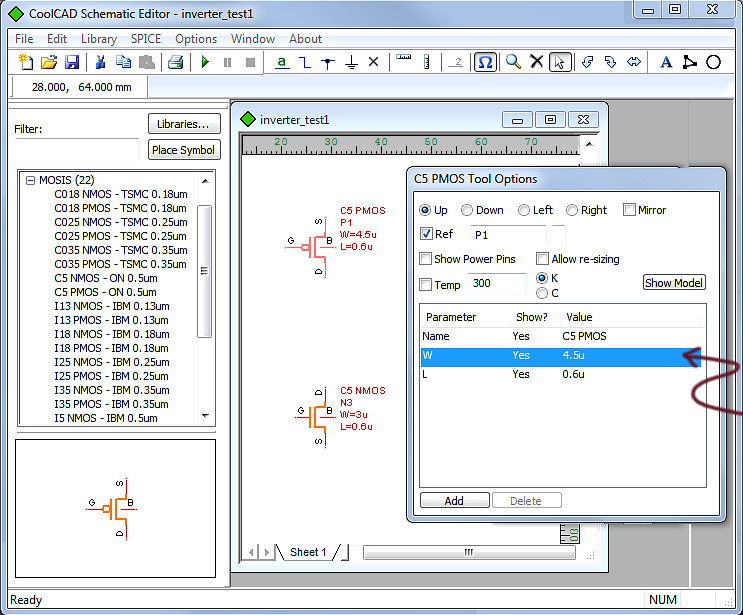
\includegraphics[width=0.55\textwidth]{./figures/getting_started_figures/SchematicEditor_ChangePMOSWidth.png}
    \caption{Changing component parameters using the \window{Options}.}
  \label{fig_schematiceditor_changePMOSwidth}
\end{SCfigure}

\begin{SCfigure}[5.0][hbt]
    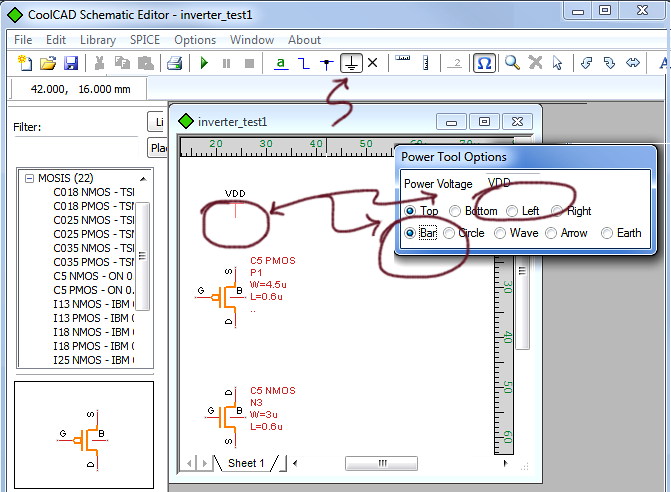
\includegraphics[width=0.55\textwidth]{./figures/getting_started_figures/SchematicEditor_addingVDD.png}
    \caption{{Adding the VDD net pin.}}
  \label{fig_schematiceditor_addVDD}
\end{SCfigure}

\mymarginnote{Power and\\ground nets} We need to add power and ground nets and voltage sources. To add the pins for the power net, we use the \menuorbutton{Power} button (marked with the earth ground symbol) or press \makekey{F4}.  The net name is set in the dialogue box; symbol rotation and type are set by the radio buttons.  Figure \ref{fig_schematiceditor_addVDD} shows the VDD pin being added. \index{Schematic Editor!power nets} For the ground net, there are two options: \index{Schematic Editor!ground net} If the \menuorbutton{Power} button option is used, the pin \textit{must} be named ``\textbf{0}", which is in fact the default name; the other option is to use the ``\textbf{Source - Ground}" component in the \textbf{Analog} library, \index{Components!ground net} as in this example circuit (see Fig. \ref{fig_schematiceditor_wiredtogether}).   \index{Schematic Editor!ground nets}

\mymarginnote{Voltage\\sources} The voltage sources are also available under the Analog library. For this example we use DC voltage sources, labelled ``SourceV - DC AC" in the program.  Figure \ref{fig_schematiceditor_wiredtogether} shows the placement, naming and parameters of these DC sources. 

%\pagebreak
\mymarginnote{Adding\\ wires} Wires are added using the \menuorbutton{Wire} button (see Fig. \ref{fig_schematiceditor_wiredtogether}) or the \makekey{F2} hotkey. \index{Schematic Editor!wiring} Click to start the wire and once in the path to turn a corner.  (The first corner-turn in a given path is also detected from the mouse movement.) The wire angle can be set in the \dial{Wire Options}.  Double-clicking after a straight extension or right-clicking at any time ends the piece.  When the wire crosses another wire, a circle appears to present the option of forming a connection with a single click.  A connection also ends the wire segment. Figure \ref{fig_schematiceditor_wiredtogether} shows the wired circuit just before the last connection is placed. (Note that the mouse scroll button or the PgUp/PgDown keys zoom in/out. This is a zoomed-in figure. The user can also pan around the design by right click-hold-dragging the mouse.)  
\begin{SCfigure}[3.0][hbt]
    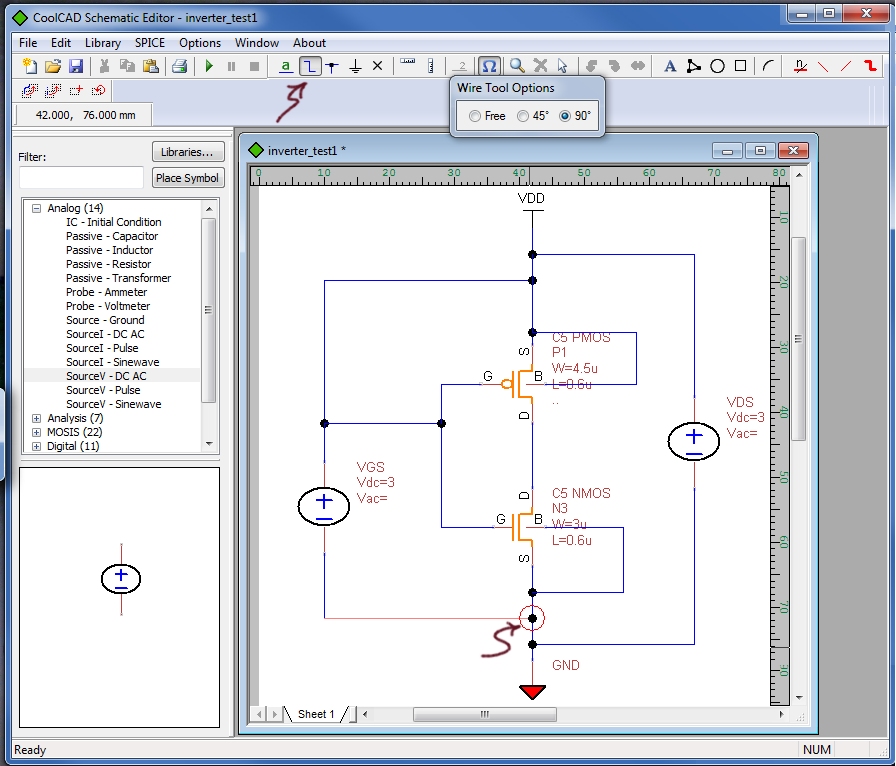
\includegraphics[width=0.55\textwidth]{./figures/getting_started_figures/SchematicEditor_addingwires.png}
    \caption{{Wired circuit.}}
  \label{fig_schematiceditor_wiredtogether}
\end{SCfigure} 


%\FloatBarrier
%\clearpage
%\newpage
%
\subsection{Analyses, Simulation and Viewing Results}

\inserttip{Do not label the net connected to the ground node or a power pin (e.g. VDD).\\Do not rely on capitalization to distinguish nets.} \mymarginnote{Labelling\\ nets} In order to measure and plot voltage signals, nets can be labelled with the Label tool (the button marked \fbox{\underline{a}}, or the \makekey{F1} hotkey).  \index{Schematic Editor!probes} For current signals, a current meter should be used.  The current meter is in the Analog library as ``Probe - Ammeter".  Figure \ref{fig_schematiceditor_sensetools} shows these elements in place and the input and output nets being labelled with \textsf{``Vin"} and \textsf{``Vout"}.  Note that the net names are \textit{not case-sensitive}. In SPICE, a net named \textsf{VGS} and one named \textsf{vgs} are the same in the netlist and if they are electrically different nets in the circuit, conflicts and errors will arise. \index{Naming nets} 

\mymarginnote{Defining\\analyses} The SPICE analysis tools are in the \textbf{``Analysis"} library.  For this example we use the \textsf{\textbf{.dc}} analysis. \index{SPICE!statements!.dc} \index{DC analysis} \index{Schematic Editor!SPICE analyses} Figure \ref{fig_schematiceditor_analysistool} shows the DC analysis setup in place.  Note especially how the voltage source to be swept is specified as ``Voltage Source1".  In this case, the common gate of the MOSFETs is being swept from 0 to 3V (the rail voltage) in 0.05V increments.

%\begin{figure}[b]
  %\centering
    %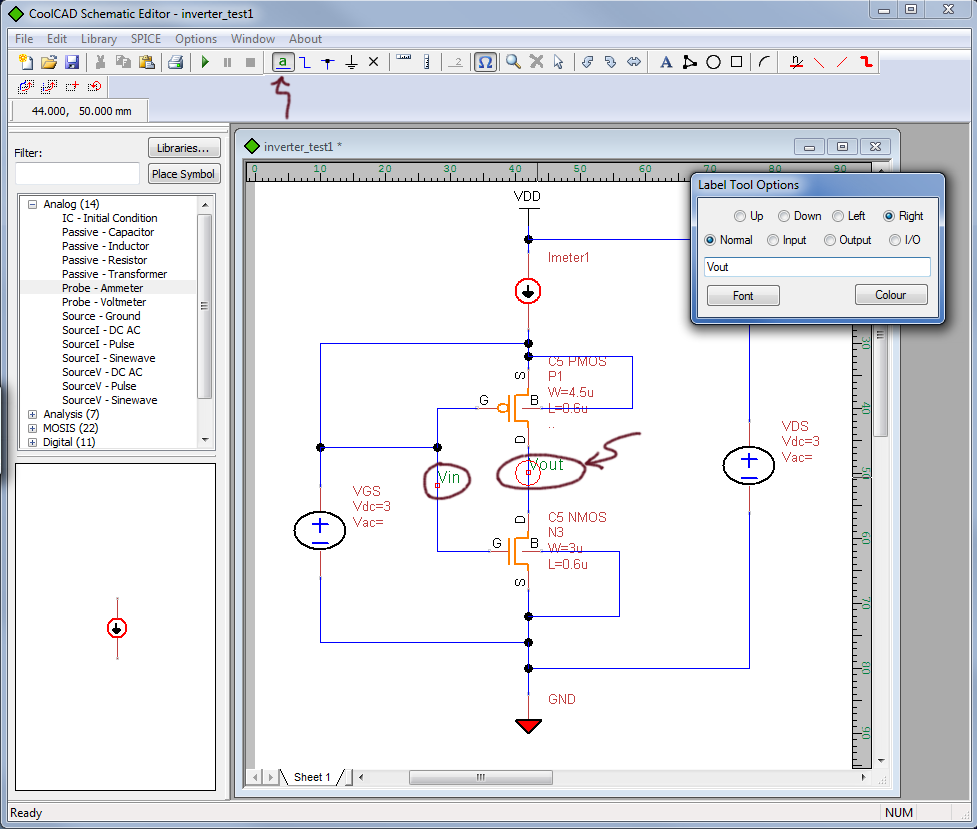
\includegraphics[width=0.55\textwidth]{./figures/getting_started_figures/SchematicEditor_labeling_and_Isense.png}
    %\caption{Inverter with input/output net labels and a current meter at the PMOS source.}
  %\label{fig_schematiceditor_sensetools}
%\end{figure} 

\begin{SCfigure}[5.0][ht]
    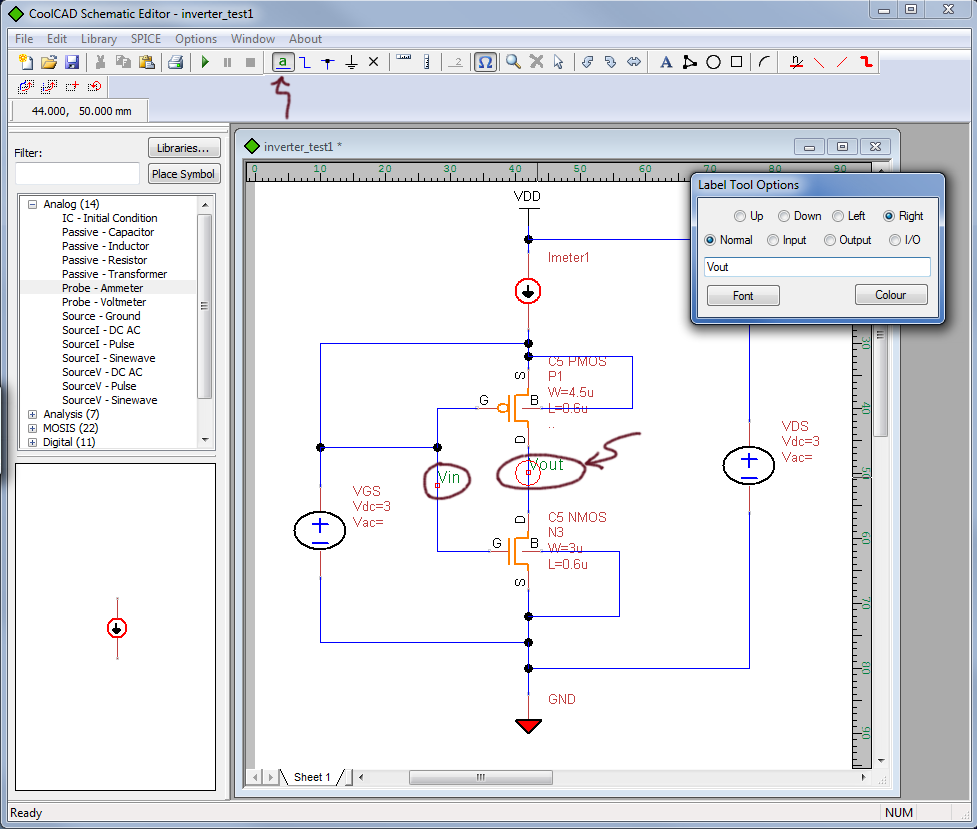
\includegraphics[width=0.55\textwidth]{./figures/getting_started_figures/SchematicEditor_labeling_and_Isense.png}
    \caption{Inverter with input/output net labels and a current meter at the PMOS source.}
  \label{fig_schematiceditor_sensetools}
\end{SCfigure} 

\mymarginnote{Saving and running} To run the analysis we first need to save the design.  The \menuorbutton{Save} button (floppy disk symbol) or the \menuitem{File}{Save} can be used.  To start the simulation, use the \menuorbutton{Run} button  (the ``play" symbol) or the \menuitem{SPICE}{Create Spice Net List and Run}.  This will create the netlist and ask for the netlist filename.  Here we use the same name as the design, \textsf{\textbf{inverter\_test1}}.  Just to see the netlist without running the simulation, use \menuitem{SPICE}{View SPICE Netlist}.  (The netlist is not editable from this view.)

\begin{SCfigure}[5.0][ht]
    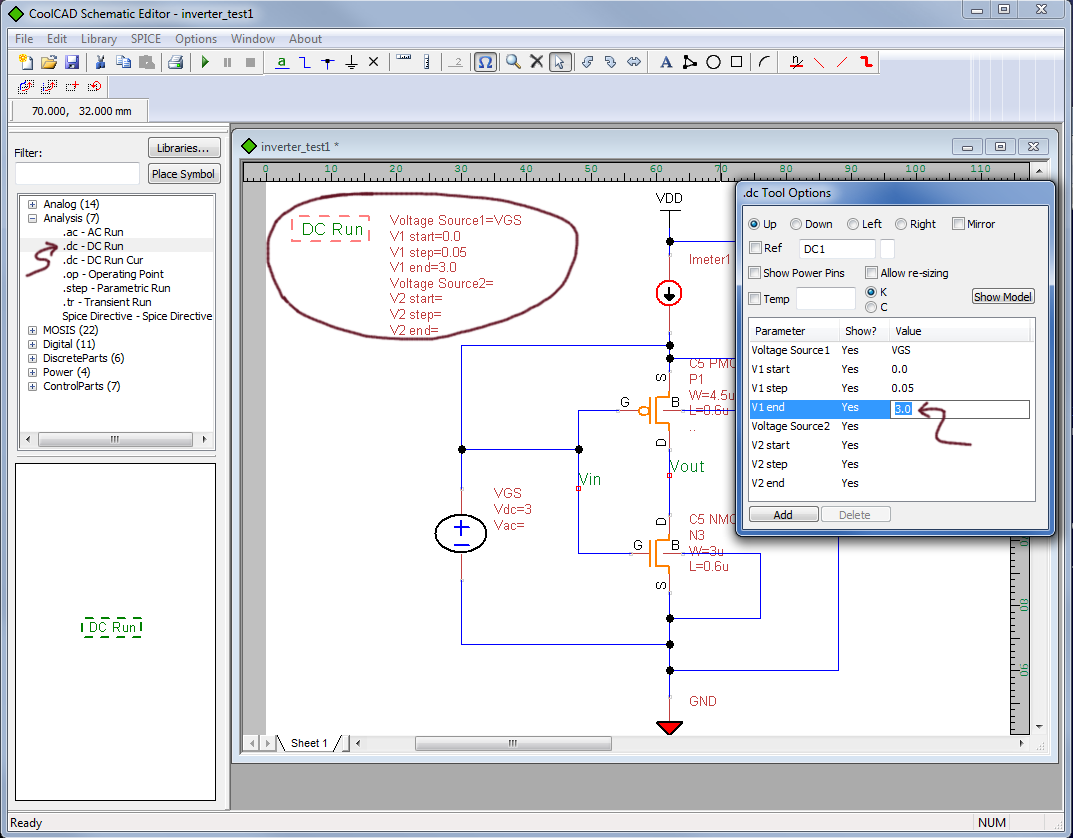
\includegraphics[width=0.55\textwidth]{./figures/getting_started_figures/SchematicEditor_DCrunadded.png}
    \caption{{DC sweep specification.}}
  \label{fig_schematiceditor_analysistool}
\end{SCfigure} 


%\FloatBarrier
%
Under the \menuitem{SPICE}{Preferences}, {CoolSPICE} can be set to automatically launch the Plotter and/or show the simulation Log File and raw data file after the simulation is complete.  By default, the "Launch Plotter" option is enabled and the options to show log/raw data file are disabled. 

\inserttip{The model paths are relative! Watch where the netlister is searching for the model cards.}\mymarginnote{Simulation\\failures due\\to path error} A common cause for simulation failure is the path specification errors for the models.  CoolSPICE comes with built-in example circuits under the folder \textsf{CoolSpice/Ckts}, symbol libraries under \textsf{Libraries/} and model cards under \textsf{Models/}.  During netlist creation, the netlister looks for the models in the \textsf{../Models/} folder (\textit{i.e.} it expects the \textsf{Models/} folder to be one level up from the circuit itself) unless the models are edited to point at an alternative location.  If the path is not where the program searches, the simulation will fail, quietly if the user has not changed the SPICE preferences to show the logfile automatically.  (If the Plotter has been set to launch automatically, a window will warn that no raw data file was found.) As shown in Fig. \ref{fig_schematiceditor_logfileerror}, the log file (which is stored in the same folder as the circuit) displays where the netlister looked for the model file.  To avoid this problem, save the designs either in the \textsf{CoolSpice/Ckts/} folder (which is created by default) or in a folder at the same path level, such as \textsf{CoolSpice/MyCircuits/}. 

\begin{SCfigure}[5.0][t]
    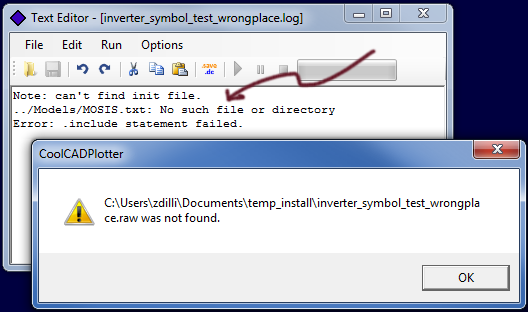
\includegraphics[width=0.55\textwidth]{./figures/getting_started_figures/SchematicEditor_modelswrongplace.png}
    \caption{Error recorded in the log file if the model for devices in the circuit are not found where expected.}
  \label{fig_schematiceditor_logfileerror}
\end{SCfigure} 

\mymarginnote{Adding\\ a trace} After the simulation is complete, the CoolCADPlotter window \index{Plotter} is automatically launched if the option is enabled as it is by default.  To view results, click the \menuorbutton{Add Trace} button (see Fig. \ref{fig_plotter_addingtraces}) or use the \menuitem{Graph}{Add Traces}. \index{Plotter!adding traces}  The only option the software will present in this example is the current trace from the current probe, as seen in the figure.

\begin{SCfigure}[5.0][ht]
    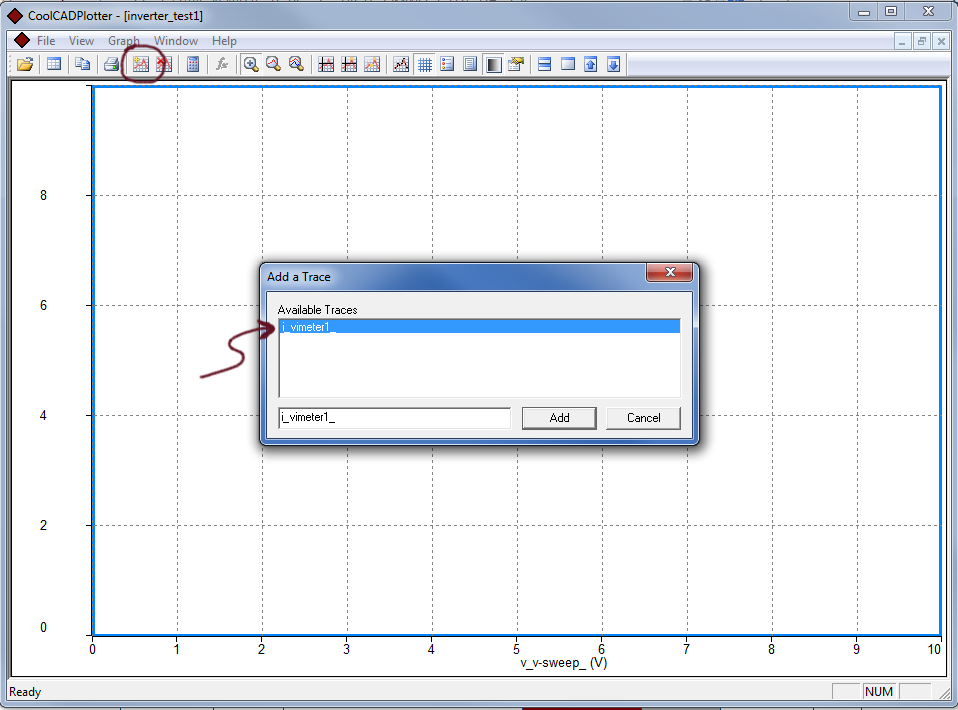
\includegraphics[width=0.55\textwidth]{./figures/getting_started_figures/Plotter_addingtrace.png}
    \caption{Adding traces to the plotter.}
  \label{fig_plotter_addingtraces}
\end{SCfigure} 

%\FloatBarrier
%\clearpage
%
\mymarginnote{Setting trace\\ and view properties, navigating} Right-clicking on the plotting area allows the user to set properties of the trace (such as color and style), move traces between panels, make measurements or use other trace tools.  Right-clicking and dragging in the plotting area pans around the plot.  \index{Plotter!trace properties} \index{Plotter!ploto navigation} Single-clicking on an axis allows the user to set axis properties such as the label, ranges and step size. \index{Plotter!axis properties} Click-and-dragging to create a rectangle in the plotting area zooms in on that area.  Double-clicking on the trace-label box which displays the trace color and name zooms out to the full trace.   Right-clicking on the trace-label box opens the trace properties. When there are multiple traces, clicking on a trace name in the legend box makes it the active trace for measurements.  When there are multiple panes, a blue frame marks the active pane.

\begin{SCfigure}[5.0][h]
  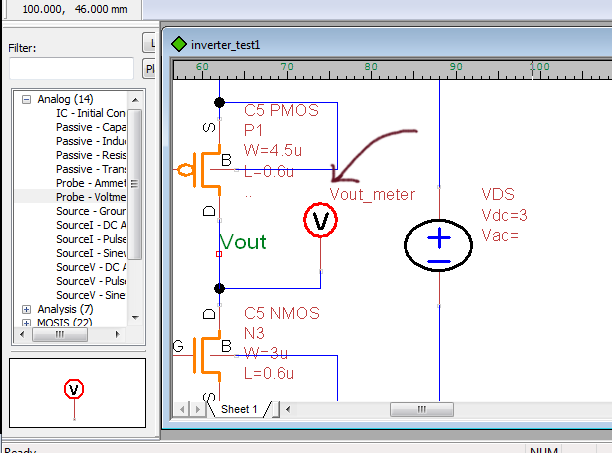
\includegraphics[width=0.55\textwidth]
	{./figures/getting_started_figures/SchematicEditor_voltageprobeadded.png}
  \caption{A voltage probe connected to the \textsf{Vout} net.}
  \label{fig_addvoltageprobe}
\end{SCfigure}

For voltage transfer function, we add a voltage probe to the schematic (the \textsf{Probe - Voltmeter} component under the Analog library) connected to the line labeled \textsf{Vout}, as shown in Fig. \ref{fig_addvoltageprobe}.  After re-running the simulation, we can now add both traces and view the current and voltage transfer functions of the inverter.  Figure \ref{fig_plotter_bothtraces} shows the Plotter window when both traces have been added.  Since one trace is from a current meter and the other from a voltage meter, they are by default plotted on separate y-axes.  Note that the legend insets can be grabbed and moved by the mouse, as was done in this example since by default they blocked the low-input-voltage part of the voltage transfer function. 

\begin{SCfigure}[5.0][h]
    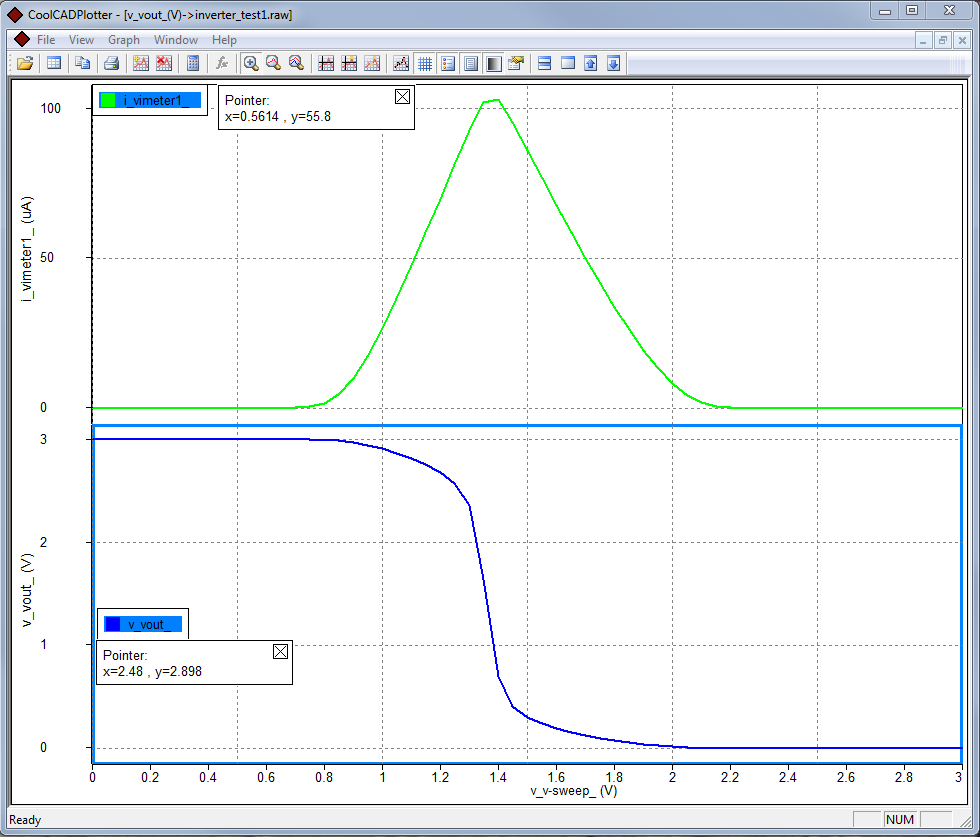
\includegraphics[width=0.55\textwidth]{./figures/getting_started_figures/Plotter_twotraces.png}
    \caption{The Plotter displaying two traces.}
  \label{fig_plotter_bothtraces}
\end{SCfigure} 

Another simulation example is given in Figure \ref{fig_transientsimexample}, where a one-stage common-source amplifier is simulated with \textsf{.tran} (transient) analysis.  Note that not $V_{in}$ but $V_{in}-1.25$ is displayed, so that the DC offset at the gate is removed to make reading the graph easier.  This is achieved using the \menuorbutton{Calculator} tool in the Plotter.

\begin{figure}[hbt]
\centering
  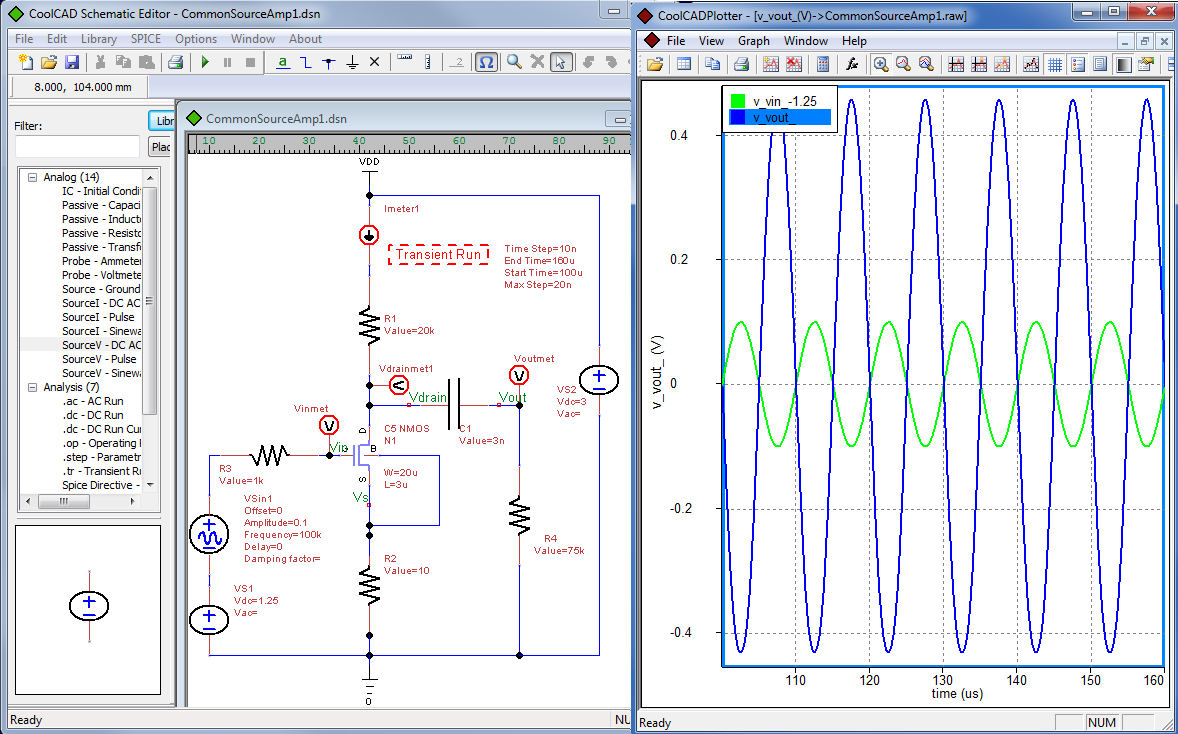
\includegraphics[width=0.55\textwidth]
	{./figures/getting_started_figures/CoolSPICE_examplesimulation_transient.png}
  \caption{A basic common-source amplifier simulated using transient analysis.}
  \label{fig_transientsimexample}
\end{figure}

The last example here in Figure \ref{fig_acsimexample} is the same CS amplifier subjected to a frequency-domain analysis using the \textsf{.ac} analysis tool.  Since the \textsf{.ac} tool in SPICE requires an AC source, note that the \textsf{SourceV - Sinewave} element in Fig. \ref{fig_transientsimexample} has been replaced with a \textsf{SourceV - DC AC} element in the new circuit.  The Plotter automatically plots the magnitude and phase of the selected traces, which allows the designer to evaluate the frequency domain characteristics of the circuit.

\begin{figure}[hbt]
\centering
  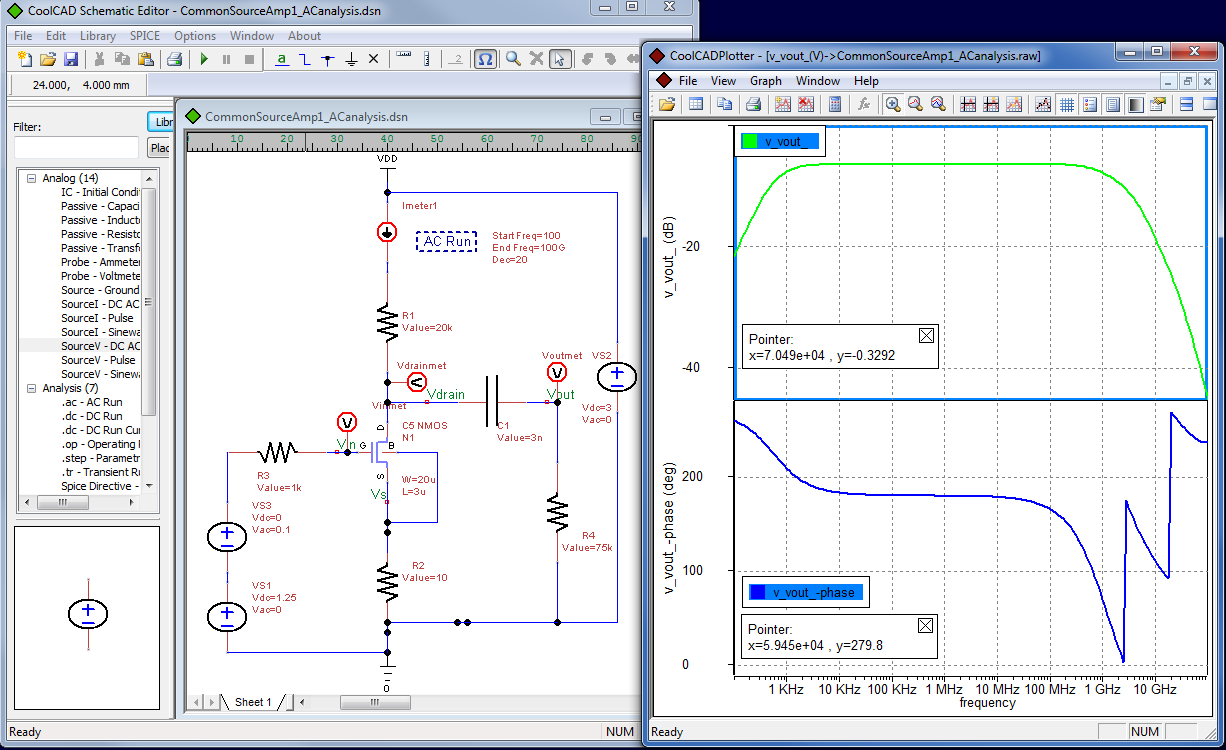
\includegraphics[width=0.55\textwidth]
	{./figures/getting_started_figures/CoolSPICE_examplesimulation_ac.png}
  \caption{A basic common-source amplifier simulated using ac analysis.}
  \label{fig_acsimexample}
\end{figure}

%\FloatBarrier
%
\subsection{Example Circuits}

Under the folder \textsf{CoolSpice/Ckts/} there are example circuits which are bundled with the program.  Running and playing around with the designs and SPICE analysis statements in these circuits is a good way to rapidly learn more about CoolSPICE and its capabilities.  As an example, Fig. \ref{fig_examplecircuitrunresult} shows the example circuit \textsf{IV\_IDVDM}, a circuit designed to run $I_{D}$-$V_{DS}$ sweeps on an TSMC 0.18 $\mu$m NMOS with $V_{GS}$ as a parameter.  Once the simulation is run as it is in the example, the curve \textsf{i\_vimeter} is available to  view in the Plotter.

\begin{figure}[hbt]
\centering
  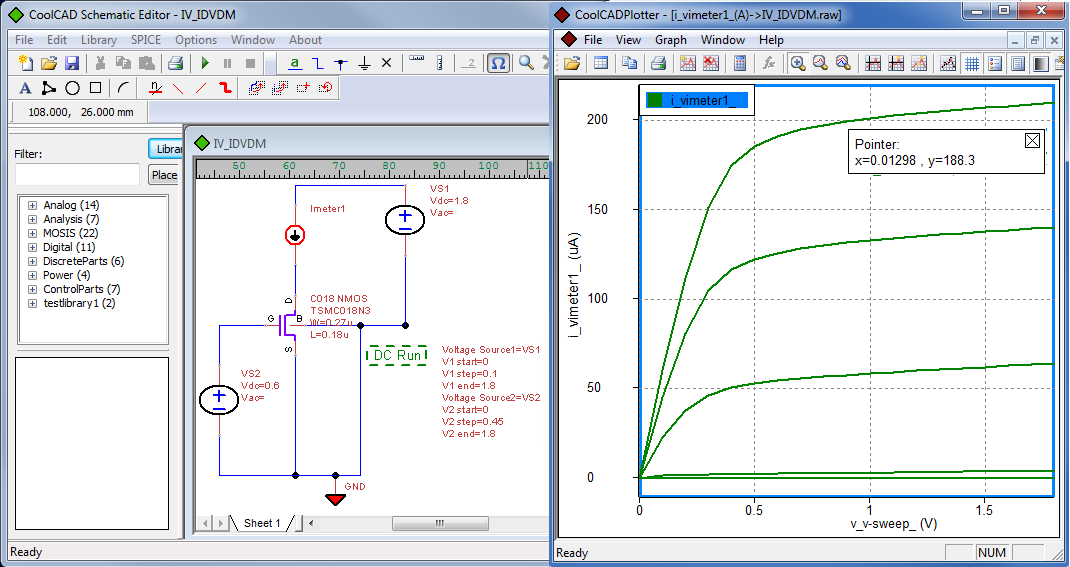
\includegraphics[width=0.55\textwidth]
	{./figures/getting_started_figures/CoolSPICE_examplecircuit_IV_IDVDM.png}
  \caption{The example circuit \textsf{IV\_IDVDM} found in the \textsf{Ckts/} directory and its run results.}
  \label{fig_examplecircuitrunresult}
\end{figure}

%\FloatBarrier
%\clearpage
%
\subsection{Creating a New Symbol for Hierarchical Designs}
\label{subsec_iags_newsymbol}

To include a circuit or subcircuit in another schematic, a symbol needs to be associated with this circuit or subcircuit. \index{Schematic Editor!new symbol creation} In this example we design the symbol for the inverter circuit.  

The \menuitem{SPICE}{Add hierarchical symbol} opens another tab in the design window.  \mymarginnote{Polygon tool}  The original circuit remains on a tab named ``Sheet 1" by default.  The polygon tool, marked in Fig. \ref{fig_schematiceditor_symbol1}, can be used to draw lines and shapes.  The ellipse, rectangle and arc tools are also available in buttons next to the polygon tool. When using the polygon tool, right-click and choose \textsf{``Finish polygon"} to stop drawing. \index{Schematic Editor!drawing tools}

\begin{figure}[hbt]
\centering
  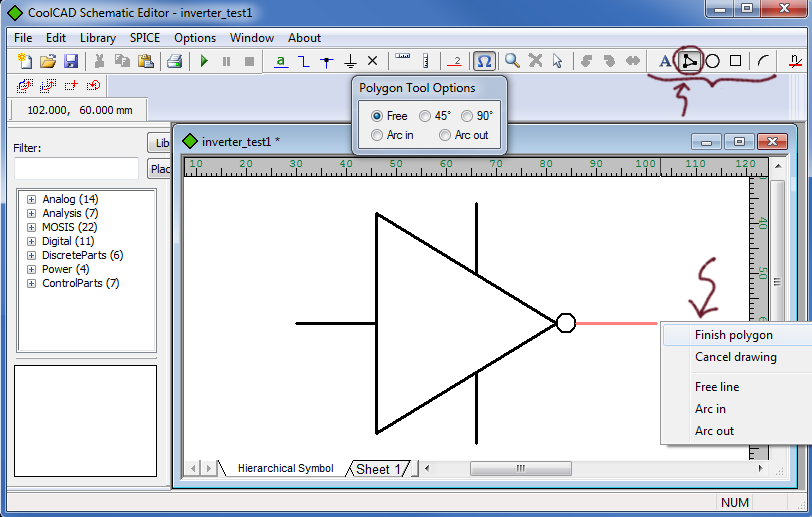
\includegraphics[width=0.55\textwidth]
	{./figures/getting_started_figures/SchematicEditor_drawingsymbol1.png}
  \caption{Creating an inverter symbol using the hierarchical symbol definition tool in the Schematic Editor.}
  \label{fig_schematiceditor_symbol1}
\end{figure}

\mymarginnote{Adding\\ symbol pins} The design itself should have labels on all the nodes which will correspond to pins in the symbol.  We first revise the design to take out the DC analysis command and the sources, since the VDD and ground pins of the inverter symbol would presumably be connected to sources in the circuit into which the inverter symbol is inserted.  Figure \ref{fig_schematiceditor_symbolandcircuit} shows, on the left, the revised circuit (note the new net names for VDD and ground) and, on the right, the corresponding symbol pins being added. \index{Schematic Editor!symbol pins} The pins are added with the \menuorbutton{Add Symbol Pin} button as marked in the figure.  Before clicking to place a pin, define the pin name, direction, graphical type and electrical type with the dialogue box.  Make sure that the electrical type fits what each pin needs to be for the circuit: In this example, \textsf{Vin} is an input pin, \textsf{Vout} is an output pin, and \textsf{VDD} and \textsf{cktgnd} are defined as input/output pins.  If unsure which type to use, it is best to pick ``input/output." 

\inserttip{Make sure to set reference names for the hierarchical symbols.}\mymarginnote{Hierarchical\\symbol\\references}Once the symbol has been saved, it can be incorporated into another circuit with the \menuitem{SPICE}{Insert another design as symbol...}. \index{Schematic Editor!using symbols}  The inverter circuit simulation results from Section are replicated using this new inverter symbol in Fig. \ref{fig_usingsymbolincircuitexample}.  Note that the reference names for inserted hierarchical symbols are \textsf{not} set automatically; nor are they incremented if you copy-paste a symbol to create multiple instances.  Set a distinct reference name for each symbol instance to avoid netlist errors.

\begin{figure}[th]
  \centering
    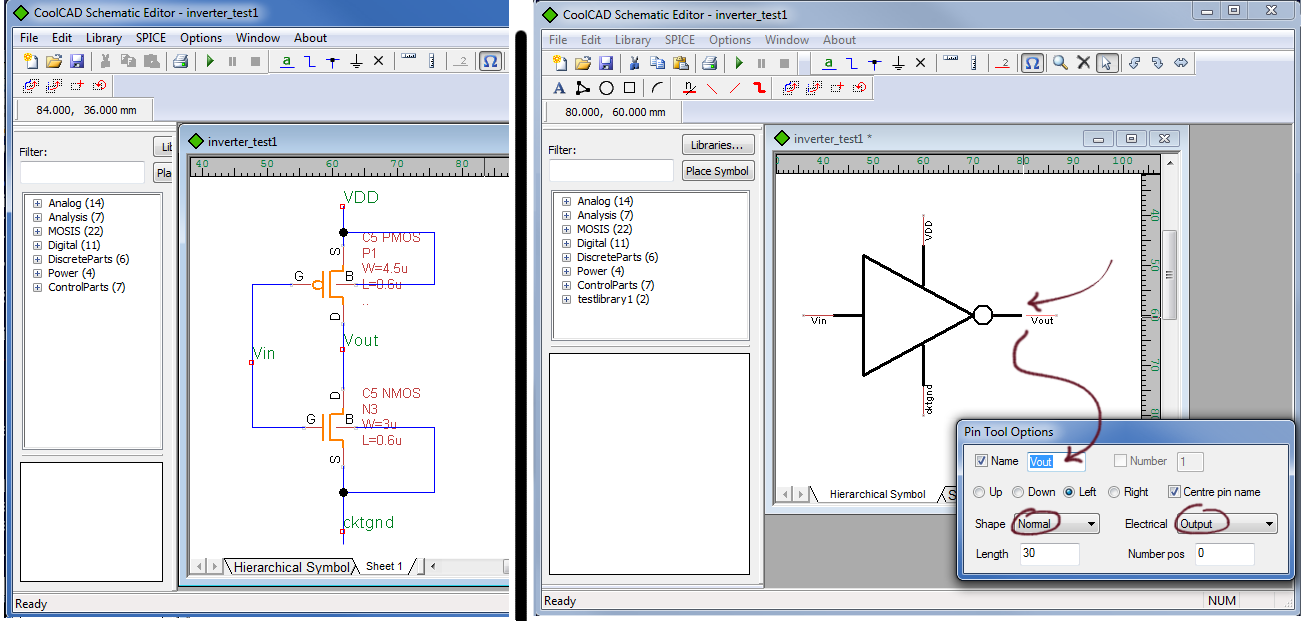
\includegraphics[width=0.55\textwidth]{./figures/getting_started_figures/SchematicEditor_revisedcircuitandsymbol2.png}
    \caption{The inverter circuit revised for representation as a hierarchical symbol (left) and pin definition in the symbol view (right).}
  \label{fig_schematiceditor_symbolandcircuit}
\end{figure} 

\begin{figure}[hbt]
  \centering
    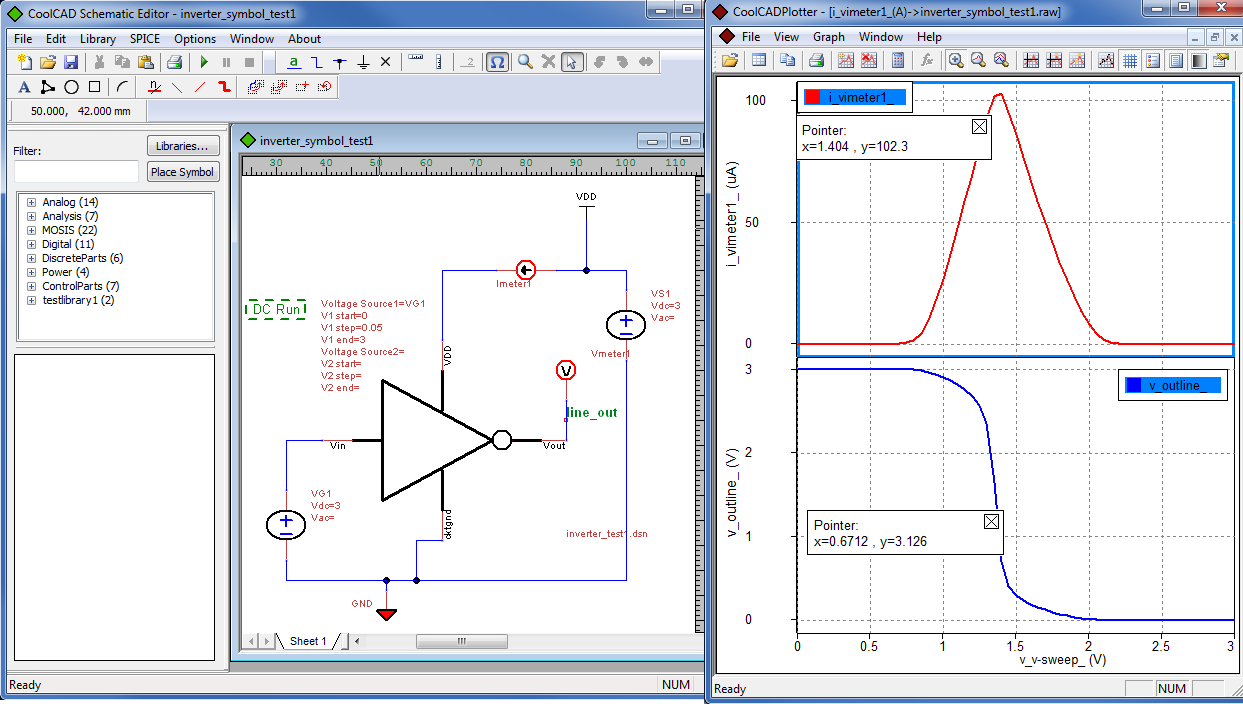
\includegraphics[width=0.55\textwidth]{./figures/getting_started_figures/CoolSPICE_invertersymbolincircuitexample2.png}
    \caption{The inverter symbol used in a simulation.}
  \label{fig_usingsymbolincircuitexample}
\end{figure} 

%\FloatBarrier
%\clearpage
%\newpage
%
\subsection{Creating New Component Models and Libraries}

In the Schematic Editor, users can access existing libraries to edit them, or add new component libraries, by the \makebutton{Libraries...} button at the top of the left-side frame (see Fig. \ref{fig_schematiceditor_accessinglibraries}). \index{Schematic Editor!component libraries!adding new components} This opens the \window{Library Setup}.  In this window, double-clicking a library or selecting it and clicking the \makebutton{Edit} button opens the symbol list for this library.  There, the user can right-click on an existing symbol to edit the symbol or perform other operations. \index{Component libraries!editing} \index{Component libraries!new library}

\begin{figure}[htb]
  \centering
    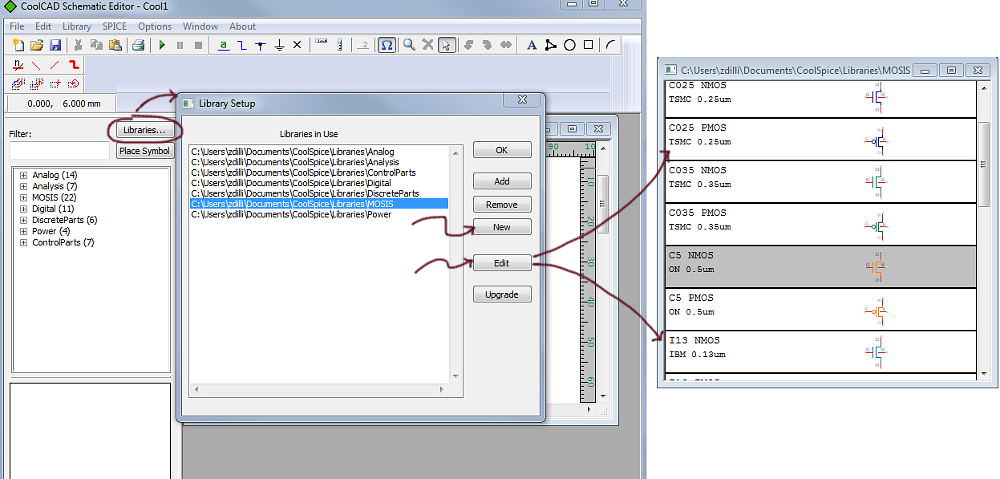
\includegraphics[width=0.55\textwidth]
		{./figures/getting_started_figures/SchematicEditor_openinglibraries.png}
    \caption{The \colorbox{lightgray}{\textcolor{black}{\textsf{\textbf{Libraries...}}}} button displays libraries and allows new ones to be created.}
  \label{fig_schematiceditor_accessinglibraries}
\end{figure} 

\mymarginnote{Creating a\\new library\\and adding\\a new\\component} As an example, we will create a new library and populate it with a new diode model.  The \makebutton{New} button in the \window{Library Setup} opens a \dial{Save As...}  for the user to set the location and name for the new library.  In this example, the library \textsf{testlibrary1.TCLib} is created and saved in a folder named \textsf{MyLibraries/} under the \textsf{CoolSpice} folder. \index{Component libraries!editing} \index{Component libraries!location} This sends the user back to the \window{Library Setup} with the new library added to the list.

We will base the new diode on the symbol and part statement of an existing diode in the \textbf{``DiscreteParts"} library. Double-clicking this library brings up the devices it contains.  Right-clicking on the \texttt{1N4148} diode, we choose \menuorbutton{Copy to}$\to$\menuorbutton{...} and pick the new library we created, as shown in Fig. \ref{fig_schematiceditor_copysymboltolibrary}.  This brings up the \dial{Update Library Symbol} box, showing the properties of the symbol just copied into the new library.

\begin{SCfigure}[5.0][bt]
  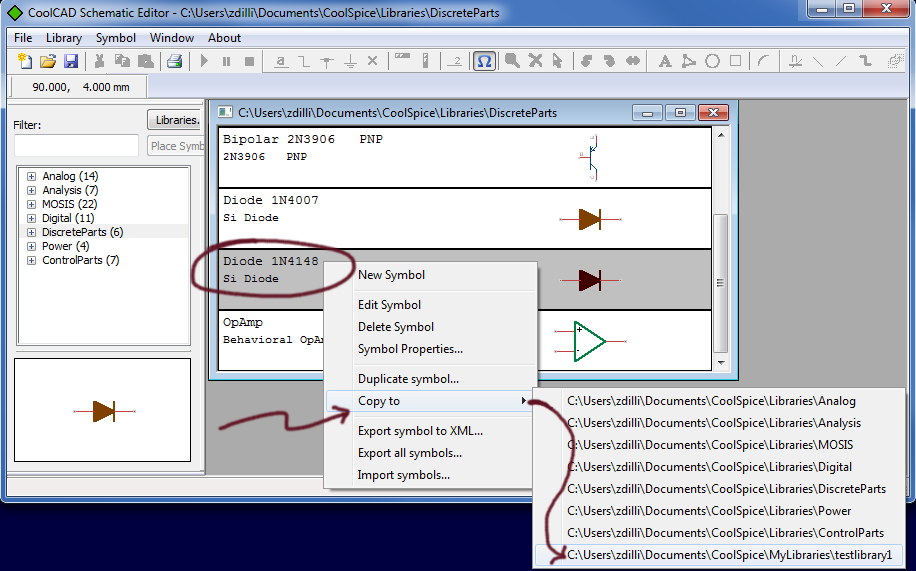
\includegraphics[width=0.55\textwidth]
	{./figures/getting_started_figures/SchematicEditor_copymodeltonewlibrary.png}
  \caption{An existing diode model is copied from the \textsf{DiscreteParts} library to the newly-created \textsf{testlibrary1} library for easy use of the symbol and the part statement.}
  \label{fig_schematiceditor_copysymboltolibrary}
\end{SCfigure}


As seen in Figure \ref{fig_schematiceditor_updatelibrarysymbol}, \textsf{Update Library Symbol} is where the attributes and associated SPICE model for components are defined.  For existing components, this window is launched by right-clicking on the symbol and choosing  \menuorbutton{``Symbol Properties..."}.  For the new component, first click on the value of the \textsf{Name} parameter and give the new name.  (Hit \menuorbutton{Tab} or \menuorbutton{Enter} for the value to be reflected in the left-side frame.)  Note that the \textsf{Reference} parameter is set as \textbf{D} since our example device is a diode.    

\begin{SCfigure}[5.0][bt]
  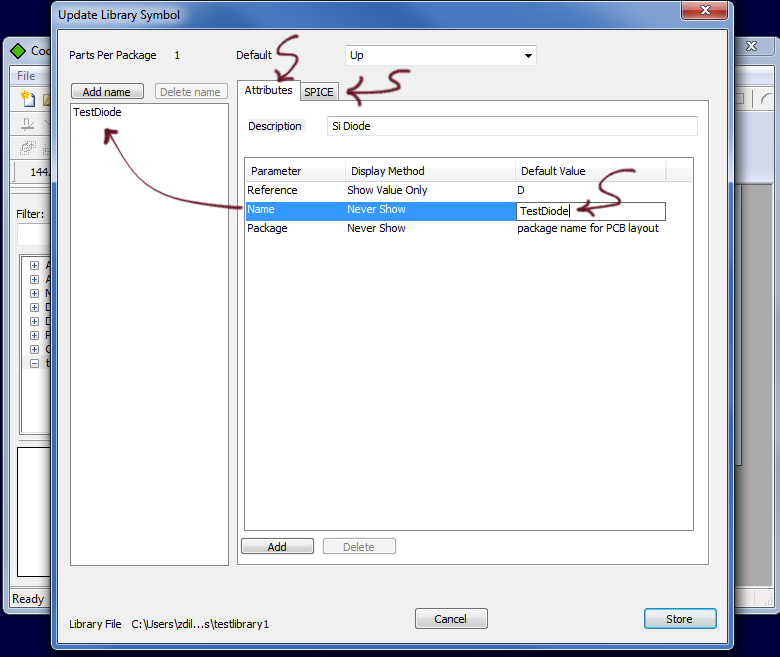
\includegraphics[width=0.55\textwidth]
	{./figures/getting_started_figures/SchematicEditor_UpdateLibrarySymbol.png}
  \caption{The name, description and other attributes of the new component are defined in the \menuorbutton{Attributes} tab of the \textsf{Update Library Symbol} {window.}}
  \label{fig_schematiceditor_updatelibrarysymbol}
\end{SCfigure}

Under the \textsf{SPICE} tab, the \textsf{``Model"} box is used to define the default \textit{part statement} the netlister uses to generate the SPICE netlist line when encountering this component. \mymarginnote{Specifying \\a device\\ model card} The \textsf{``Prologue"} or \textsf{``Epilogue"} boxes are used to define the \textsf{.include} statement which points to the model card. \index{SPICE!statements!.include} It is necessary to fill only one of these two; the netlister puts the \textsf{.include} statement either to the very beginning or the very end of the netlist depending on which one has been used.  Since we copied a diode component, we do not need to edit anything in the \textsf{Model} box part statement except the model name (see Fig. \ref{fig_schematiceditor_definingmodel}). 

\begin{SCfigure}[5.0][bt]
  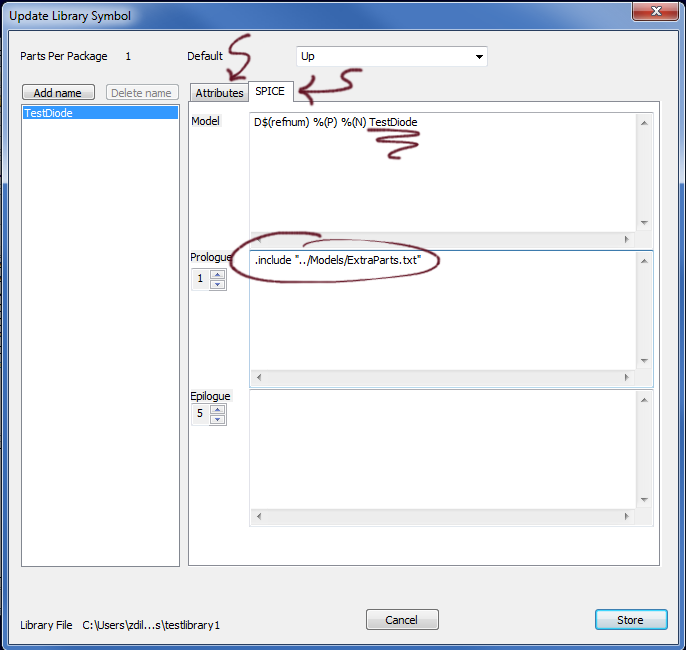
\includegraphics[width=0.55\textwidth]
	{./figures/getting_started_figures/SchematicEditor_enteringthemodel.png}
  \caption{The part statement and \textsf{.include} statement pointing to the file which includes the \textsf{.model} statement for the device are defined in the \textsf{SPICE} tab of the {\textsf{Update Library Symbol}} window.}
  \label{fig_schematiceditor_definingmodel}
\end{SCfigure}

The model name should match the model card (\textsf{.model} statement) in the text file specified by the \textsf{.include} statement in the \textsf{Prologue} or \textsf{Epilogue} box.  For this example, the contents of the text file {\textsf{../Models/ExtraParts.txt}} have been reproduced below.
\vspace{\parskip}

\noindent\begin{minipage}{\textwidth}
\begin{center}\small{
\texttt{.model TestDiode  D(Is=5.84n N=1.94 Rs=.7017 Ikf=44.17m Xti=3 
Eg=1.11\\+Cjo=.95p M=.55 Vj=.75 Fc=.5 Isr=11.1n Nr=2.09 Bv=100 Ibv=100u Tt=11.1n)}}
\end{center}
\end{minipage}
\inserttip{Note that the model name (\texttt{TestDiode}) specified at the end of the part statement in the \textsf{Model} box in Fig. \ref{fig_schematiceditor_definingmodel}.} 

Click \makebutton{Store} to save the symbol attributes and SPICE information and return to the symbol display window. The new component can now be used in the Schematic Editor. The new library appears in the library list and includes and the new component (See Fig. \ref{fig_schematiceditor_newdeviceavailable}). 

Another method to specify the component SPICE model is to write out the \textsf{.model} statement in the \textsf{Prologue} or \textsf{Epilogue} dialog box instead of putting it in a text file and pointing to the file with a \textsf{.include} statement as above.  However, the \textsf{.include} method has the advantage that it is possible to incorporate more than one \textsf{.model} statement in a text file.  Then, when defining the models for multiple components within the same library, the same \textsf{.include} statement works for all. This helps with organization.  For instance, Fig. \ref{fig_schematiceditor_mosfetcopyexample} shows another new device, this time a MOSFET, defined in the same library by the copying method described above.  For it to work correctly, the file \textsf{../Models/ExtraParts.txt} should now also include an NMOS \textsf{.model} statement with the model name ``generic018nmos."

It is also possible to edit existing libraries, point existing models to new \textsf{.model} statements \textit{etc.} by starting with the \makebutton{Libraries} button as above. \mymarginnote{Editing\\existing\\component\\models}However,  note that if the model for a component with existing instances in the design is changed, either by pointing it to a new model card file by editing the \textsf{.include} statement or by editing the \textsf{.model} statement in the model card text file, \textit{only new instances of it will use the new model in the netlist.}  Existing instances will have to be deleted and replaced to be associated with the modified model. \inserttip{The netlist creator does not check if models are up to date with existing instances of components! If you changed a model, replace the instances to apply the change to everything.}  

% \vfill
% \clearpage
% \pagebreak

\begin{SCfigure}[5.0][th]
	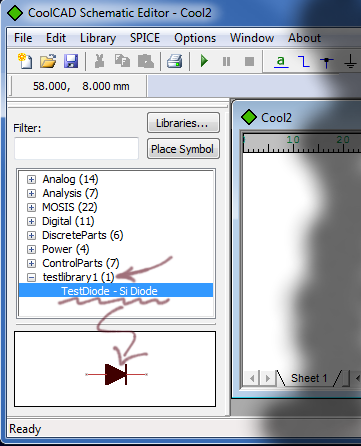
\includegraphics[width=0.25\textwidth]
	{./figures/getting_started_figures/SchematicEditor_NewLibraryDeviceAvailable.png}
  \caption{The new library and component (with its symbol and model) are now available for use in schematics.}
  \label{fig_schematiceditor_newdeviceavailable}
\end{SCfigure}

\begin{SCfigure}[5.0][bh]
	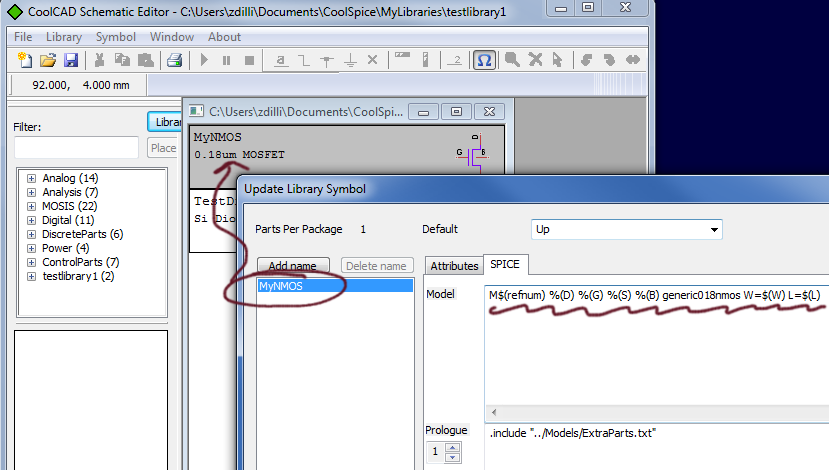
\includegraphics[width=0.7\textwidth]
	{./figures/getting_started_figures/SchematicEditor_MOSFETmodelexample.png}
  \caption{The part statement for a MOSFET defined in the new library by copying the MOSFET symbol from the MOSIS library.}
  \label{fig_schematiceditor_mosfetcopyexample}
\end{SCfigure}

%\FloatBarrier
%\newpage
%\pagebreak
%\clearpage
%
\section{References and Further Reading}

\begin{enumerate}

\item CoolCAD CoolSPICE, http://coolcadelectronics.com/coolspice/, last visited October 2014.

\item WinSCP, http://winscp.net, last visited October 2014.

\item List of SPICE device codes, http://www.ecircuitcenter.com/SPICEsummary.htm\#devices, last visited October 2014.


\end{enumerate}
